%compile with pdflatex on papeeria

\documentclass[a4paper,12pt]{article}
\usepackage{fancyhdr}
\usepackage{fancyheadings}
\usepackage[ngerman,german]{babel}
\usepackage{german}
\usepackage[utf8]{inputenc}
%\usepackage[latin1]{inputenc}
\usepackage[active]{srcltx}
%\usepackage{algorithm}
%\usepackage[noend]{algorithmic}
\usepackage{amsmath}
\usepackage{amssymb}
\usepackage{amsthm}
\usepackage{bbm}
\usepackage{enumerate}
\usepackage{graphicx}
\usepackage{ifthen}
\usepackage{listings}
\usepackage{enumitem}
%\usepackage{struktex}
\usepackage{hyperref}
\usepackage{tikz}
\usepackage{float}
\usepackage{subcaption}
\usepackage{array}
\captionsetup{compatibility=false}
\captionsetup[subfigure]{labelformat=empty}

\usepackage{pgfplots}
\pgfplotsset{compat=1.15}
\usepackage{mathrsfs}
\usetikzlibrary{arrows}

\definecolor{ccqqqq}{rgb}{0.8,0,0}
\definecolor{kolorwykresu}{rgb}{0.07,0.04,0.56}

\pagenumbering{gobble}

\usepackage{tabularray}
\usepackage{multirow}
\usepackage{booktabs,tabularx}
\renewcommand\tabularxcolumn[1]{m{#1}}% for vertical centering text in X column

\newcolumntype{L}[1]{>{\raggedright\let\newline\\\arraybackslash\hspace{0pt}}m{#1}}
\newcolumntype{C}[1]{>{\centering\let\newline\\\arraybackslash\hspace{0pt}}m{#1}}
\newcolumntype{R}[1]{>{\raggedleft\let\newline\\\arraybackslash\hspace{0pt}}m{#1}}

\newcolumntype{Y}{>{\centering\arraybackslash}X}

%%%%%%%%%%%%%%%%%%%%%%%%%%%%%%%%%%%%%%%%%%%%%%%%%%%%%%
%%%%%%%%%%%%%% EDIT THIS PART %%%%%%%%%%%%%%%%%%%%%%%%
%%%%%%%%%%%%%%%%%%%%%%%%%%%%%%%%%%%%%%%%%%%%%%%%%%%%%%
\newcommand{\Fach}{1. Klausur aus der Mathematik (A)}
\newcommand{\Name}{}
\newcommand{\datum}{}
\newcommand{\Matrikelnummer}{}
\newcommand{\Semester}{Q11/1}
\newcommand{\Uebungsblatt}{} %  <-- UPDATE ME
%%%%%%%%%%%%%%%%%%%%%%%%%%%%%%%%%%%%%%%%%%%%%%%%%%%%%%
%%%%%%%%%%%%%%%%%%%%%%%%%%%%%%%%%%%%%%%%%%%%%%%%%%%%%%

\setlength{\parindent}{0em}
\topmargin -1.0cm
\oddsidemargin 0cm
\evensidemargin 0cm
\setlength{\textheight}{9.2in}
\setlength{\textwidth}{6.0in}

%%%%%%%%%%%%%%%
%% Aufgaben-COMMAND
\newcommand{\Aufgabe}[1]{
  {
  \vspace*{0.5cm}
  \textsf{\textbf{Aufgabe #1}}
  \vspace*{0.2cm}
  
  }
}
%%%%%%%%%%%%%%
\hypersetup{
    pdftitle={\Fach{}: Übungsblatt \Uebungsblatt{}},
    pdfauthor={\Name},
    pdfborder={0 0 0}
}

\lstset{ %
language=java,
basicstyle=\footnotesize\tt,
showtabs=false,
tabsize=2,
captionpos=b,
breaklines=true,
extendedchars=true,
showstringspaces=false,
flexiblecolumns=true,
}

\title{Übungsblatt \Uebungsblatt{}}
\author{\Name{}}

\begin{document}

\fancyhead{}
\fancyhead[C]{
\includegraphics[height=2.5cm]{lukasLogo.png}
\vspace{2cm}
}

\thispagestyle{fancy}

\lhead{
%\vspace{1cm}
  \sf \LARGE \Fach{} %\small \Name{} - \Matrikelnummer{}
}
\rhead{\sf \Semester{}   \datum{}}

\vspace*{0.2cm}

\vspace{4cm}
Alle Lösungen müssen mit Nebenrechnungen und Begründungen nachvollziehbar sein!

%\rhead{\sf \Semester{} }
\vspace*{0.2cm}

%\begin{center}
%%\LARGE \sf \textbf{Übungsblatt \Uebungsblatt{}}
%\end{center}
%\vspace*{0.2cm}

%%%%%%%%%%%%%%%%%%%%%%%%%%%%%%%%%%%%%%%%%%%%%%%%%%%%%%
%% Insert your solutions here %%%%%%%%%%%%%%%%%%%%%%%%
%%%%%%%%%%%%%%%%%%%%%%%%%%%%%%%%%%%%%%%%%%%%%%%%%%%%%%

\vspace{1cm}
  Name: \underline{\hspace{7cm}}
  \hfill
  Datum: \underline{\hspace{4cm}}

%\vspace{0,5cm}Die Rechenwege müssen nachvollziehbar sein!
%
%\vspace{0,5cm} {TEIL A} - ohne Hilfsmittel - Bearbeitungszeit 30 Minuten
\vspace {2cm}
% 
%GEOMETRIE


\begin{center}
  \begin{tblr}{
      width=1\linewidth,
      colspec = {Q[c,6em]Q[c,4em]Q[c,4em]Q[c,4em]Q[c,4em]Q[c,4em]Q[c,6em]},
      rowspec = {Q[m]Q[m]Q[m]Q[m]Q[m]Q[m]Q[m]},
      colsep = 0mm,
      %row{1} = {2em,azure2,fg=white,font=\large\bfseries\sffamily},
      row{1} = {2em,font=\large\bfseries\sffamily},
      hlines, vlines,
    }
    \textbf{Aufgabe} & \textbf{1} & \textbf{2} & \textbf{3} & 
    \textbf{4} & \textbf{5} & \textbf{Gesamt} \\
    {Mögliche \\ Punkte} & {6} & {17} & {6} & 6 & 7 & 42 \\
    {Erreichte \\ Punkte} &  &  &  &  &  &  \\
  \end{tblr}
\end{center}

\vspace{5cm}
%\centerline{\huge\bfseries\sffamily Viel Erfolg !!!}

\newpage


\Aufgabe{1: (6BE)}
Entscheiden Sie, ob die folgenden Aussagen wahr oder falsch sind. Begründen Sie jeweils in einem Satz die falschen Aussagen. (Achtung: für fehlende oder falsche Angaben werden Punkte abgezogen!)\\

Gegeben ist die Funktion 
\[f: x \rightarrow \frac{3x-6}{(x+3)^2(x-2)}\]

\begin{enumerate}[label={\alph*)}]
  \item Die Definitionsmenge von $f$ ist $D_f = \{-3; 2\}$.
  \item Der Graph $G_f$ schneidet die $y$-Achse oberhalb des Ursprungs.
  \item Der Graph $G_f$ hat eine hebbare Definitionslücke.
  \item Die Funktion $f$ hat einen Pol mit Vorzeichenwechsel.
  \item Der Punkt $P(-1|2,25)$ liegt auf $G_f$.
  \item Die Wertemenge ist $W_f = ]0; \infty[$.
\end{enumerate}

\vspace{2cm}
\Aufgabe{2: (2BE + 4BE + 5BE + 3BE + 3BE)}
Gegeben ist die Funktion $f$ mit
\[ f(x) = \frac{4x^2+1}{x} = 4x + \frac{1}{x} \]
\begin{enumerate}[label={\alph*)}]
  \item Bestimmen Sie die Definitionsmenge und die Schnittpunkte mit den Koordinatenachsen.
  \item Ermitteln Sie das Verhalten an den Grenzen des Definitionsbereichs.\\
    Geben Sie die Gleichungen aller Asymptoten an.
  \item Bestimmen Sie Art und Lage des Extrempunkts von $G_f$.
  \item Bestimmen Sie Krümmungsverhalten und Lage des eventuellen Wendepunkts von $G_f$.
  \item Skizzieren Sie unter Verwendung aller bisherigen Ergebnisse den Graphen von $f$.
\end{enumerate}

\newpage
\Aufgabe{3: (3BE + 3BE)}

\addtolength{\topmargin}{-6.0pt}
\setlength{\headheight}{18.0pt}

\begin{enumerate}[label={\alph*)}]
  \item Gegeben ist die Funktion $f$ mit 
    \[ f(x) = x^2+3x-1 \]\\
    Ermitteln Sie mit Hilfe des Differentialquotienten die Ableitung der Funktion $f(x)$ an der Stelle $x=-2$.
    \item Skizzieren Sie zum gegebenen Graph der Funktion $h$ die zugehörige Ableitungsfunktion $h'$ (direkt im gegebenen Koordinatensystem)
\end{enumerate}

\begin{center}
\begin{tikzpicture}[line cap=round,line join=round,>=triangle 45,x=1cm,y=1cm,scale=0.95]
\begin{axis}[
x=1cm,y=1cm,
axis lines=middle,
ymajorgrids=true,
xmajorgrids=true,
xmin=-6.713302863837152,
xmax=6.552502227713441,
ymin=-8.69329981739455,
ymax=8.669141217180235,
xtick={-6,-5,...,4,5,6},
ytick={-8,-7,...,8},]
\clip(-4.713302863837152,-8.69329981739455) rectangle (4.552502227713441,9.069141217180235);
\draw[line width=2pt,color=kolorwykresu,smooth,samples=100,domain=-2.713302863837152:4.552502227713441] plot(\x,{0.2*((\x)+2)*((\x)-1)^(3)*((\x)-3)});
\begin{scriptsize}
\draw[color=kolorwykresu] (-1.922828743601838,-8.201389315429992) node {$h$};
\end{scriptsize}
\end{axis}
\end{tikzpicture}
\end{center}


%\begin{figure}[h!]
%  \begin{center}
%    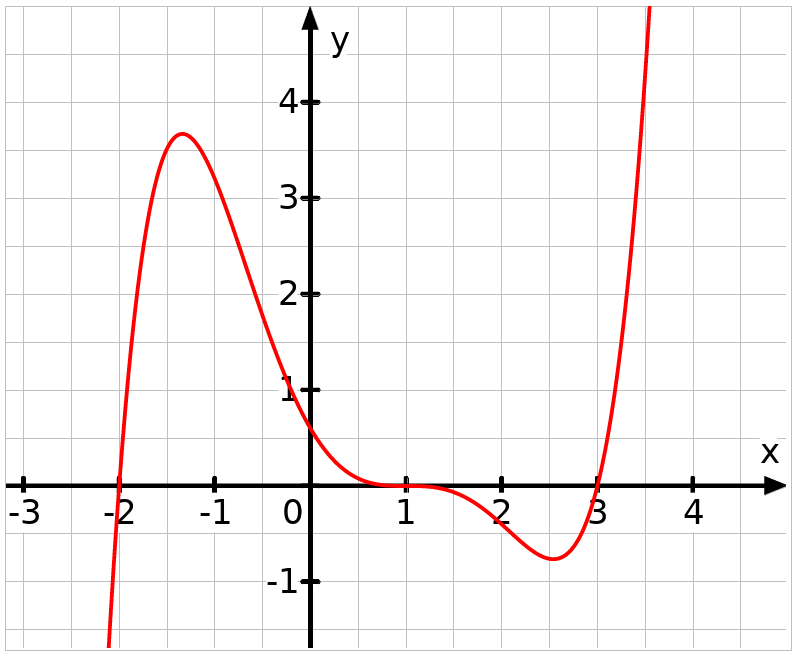
\includegraphics[width=0.9 \linewidth]{Q11_1KlausurJanuar2022_1.png}
%  \end{center}
%\end{figure}


\newpage
\enlargethispage{4cm}
\Aufgabe{4: (2BE + 4BE)}
Gegeben ist die Funktion 
\[f:x \rightarrow \frac{x^2-a}{x^2-b} \quad \text{mit $a\neq b$}\]

\begin{enumerate}[label={\alph*)}]
  \item Geben Sie einen Wert für $b$ an, so dass die Funktion $f$ für alle reellen Zahlen definiert ist. Erklären Sie kurz Ihre Entscheidung.
  \item Bestimmen Sie die Nullstellen von $f$ in Abhängigkeit von $a$. (Fallunterscheidung!)
\end{enumerate}

\Aufgabe{5: (4BE + 3BE)}
\noindent
\begin{minipage}{0.6\textwidth}%\raggedleft
Bei einem Rennen 1999 in Silverstone versagten bei Michael Schumacher Bremsen und Lenkung vor Einfahrt in die Stowe-Kurve. Der Streckenverlauf wird durch den Graph der Funktion $f$ mit
\[f(x)=-\frac{1}{3}x^2+3 \]
  angenähert, sein Wagen verlässt die Fahrbahn an der Stelle $x_0 = -3$ (Skizze!).
\end{minipage}
\hfill%
\begin{minipage}{0.3\textwidth}% adapt widths of minipages to your needs
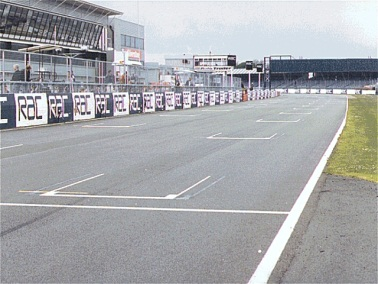
\includegraphics[width=\linewidth]{Q11_1KlausurJanuar2022_3.png}
\end{minipage}%


%\begin{figure}[h!]
%  \begin{center}
%    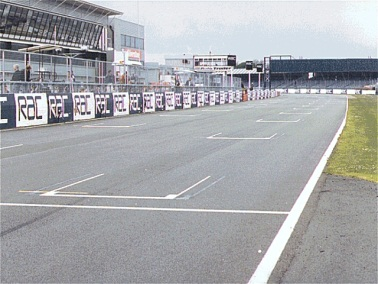
\includegraphics[width=0.4 \linewidth]{Q11_1KlausurJanuar2022_3.png}
%  \end{center}
%\end{figure}

\begin{enumerate}[label={\alph*)}]
  \item Bestimmen Sie die Gleichung der Funktion, die den weiteren Fahrtverlauf nach dem Versagen der Bremsen und der Lenkung beschreibt.\\
    \\
    Im Punkt $A(3|12)$ trifft der Ferrari auf die aufgestapelten Autoreifen, die den Aufprall auf die Mauer dämpfen sollen. Beim Aufprall fliegt das linke Vorderrad im rechten Winkel zur Aufprallrichtung davon.
  \item Bestimmen Sie die Gleichung der Funktion, die die Flugbahn des Reifens beschreibt.
\end{enumerate}

\vspace{3cm}

\centerline{Viel Erfolg}
%\enlargethispage{2\baselineskip}

%\addtolength{\voffset}{-2cm}




%\begin{tikzpicture}
%\draw [very thin, black, step=0.5cm] (0,0) grid +(15,18);
%\end{tikzpicture}


\newpage
\Aufgabe{1: Musterlösung}
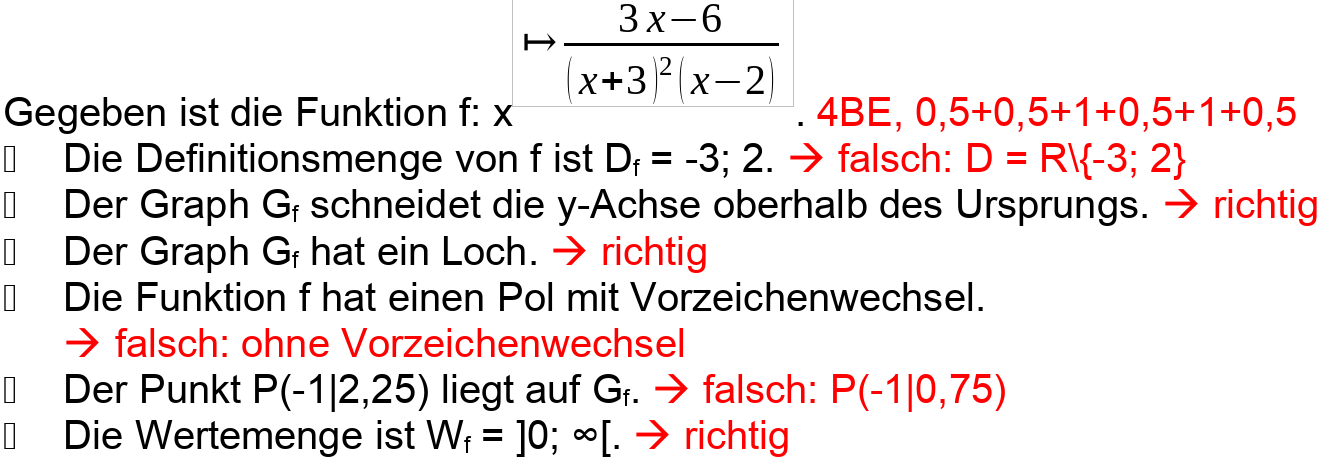
\includegraphics[width=\linewidth]{Q11_1KlausurJanuar2022_ml1.png}

\Aufgabe{2: Musterlösung}
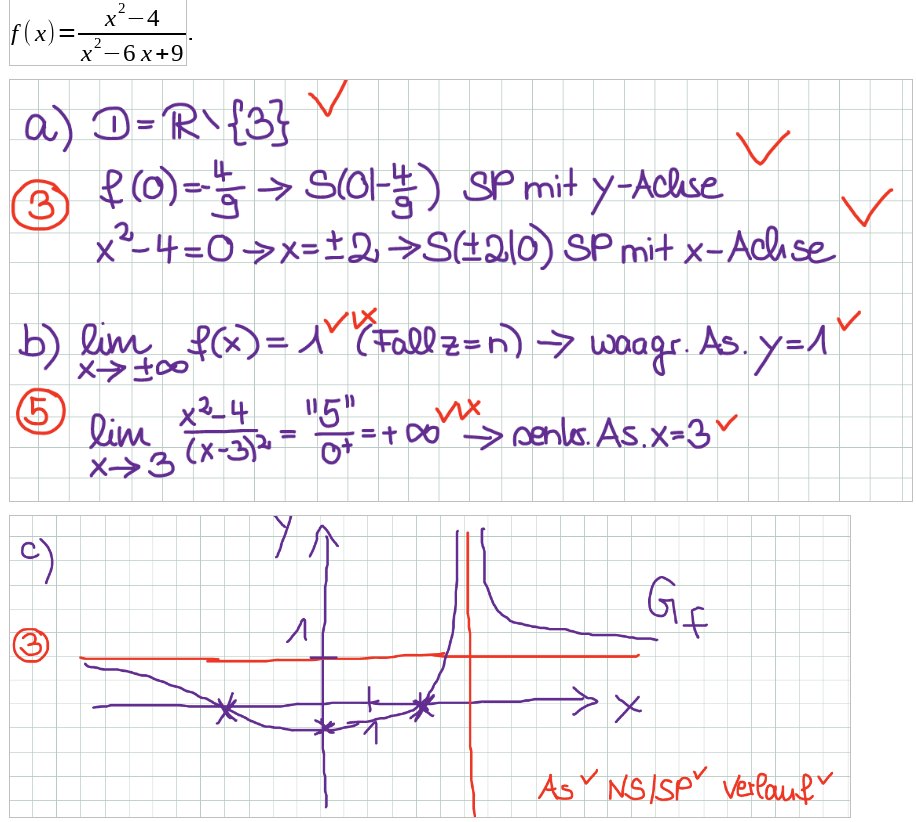
\includegraphics[width=\linewidth]{Q11_1KlausurJanuar2022_ml2.png}

\newpage
\Aufgabe{3: Musterlösung}
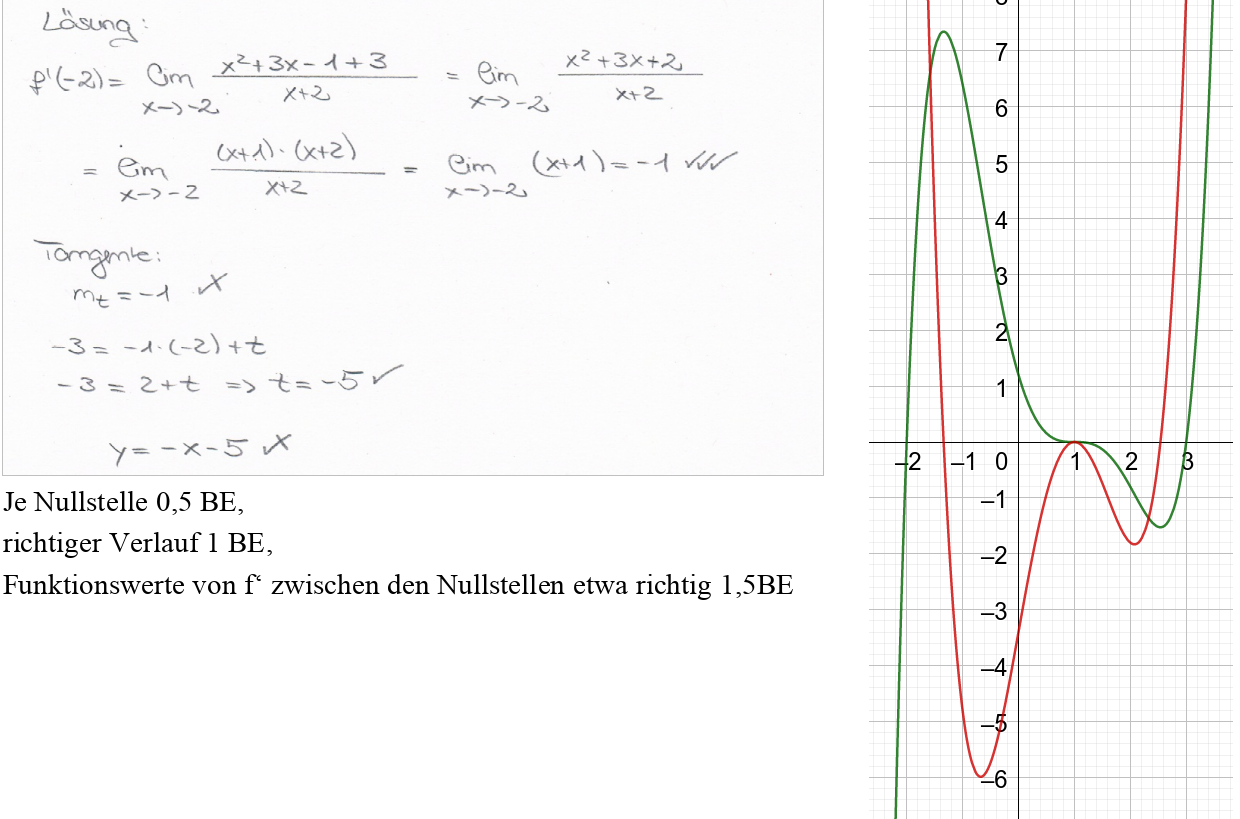
\includegraphics[width=\linewidth]{Q11_1KlausurJanuar2022_ml3a.png}

\Aufgabe{4: Musterlösung}
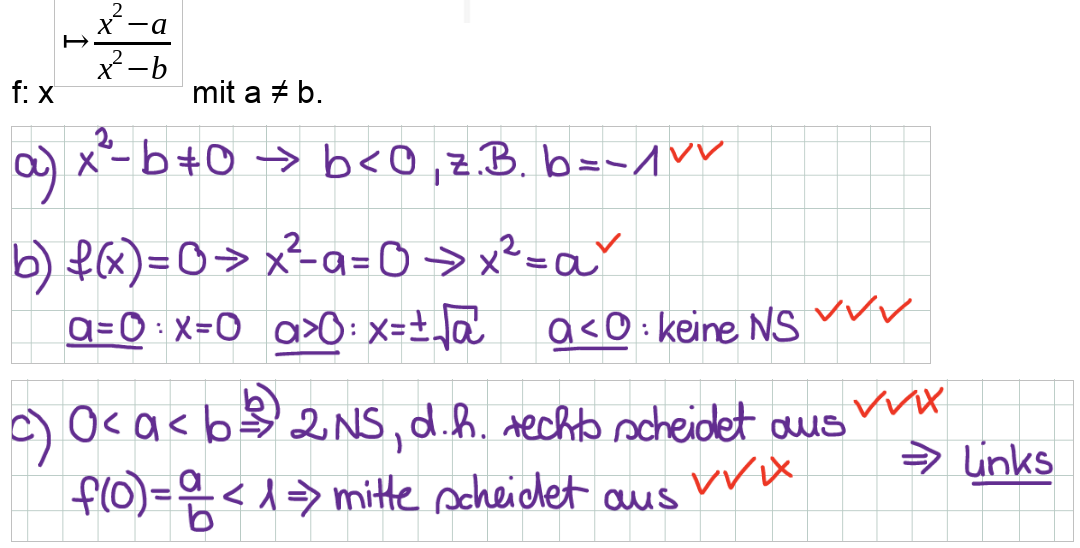
\includegraphics[width=\linewidth]{Q11_1KlausurJanuar2022_ml4.png}

\newpage
\Aufgabe{5: Musterlösung}
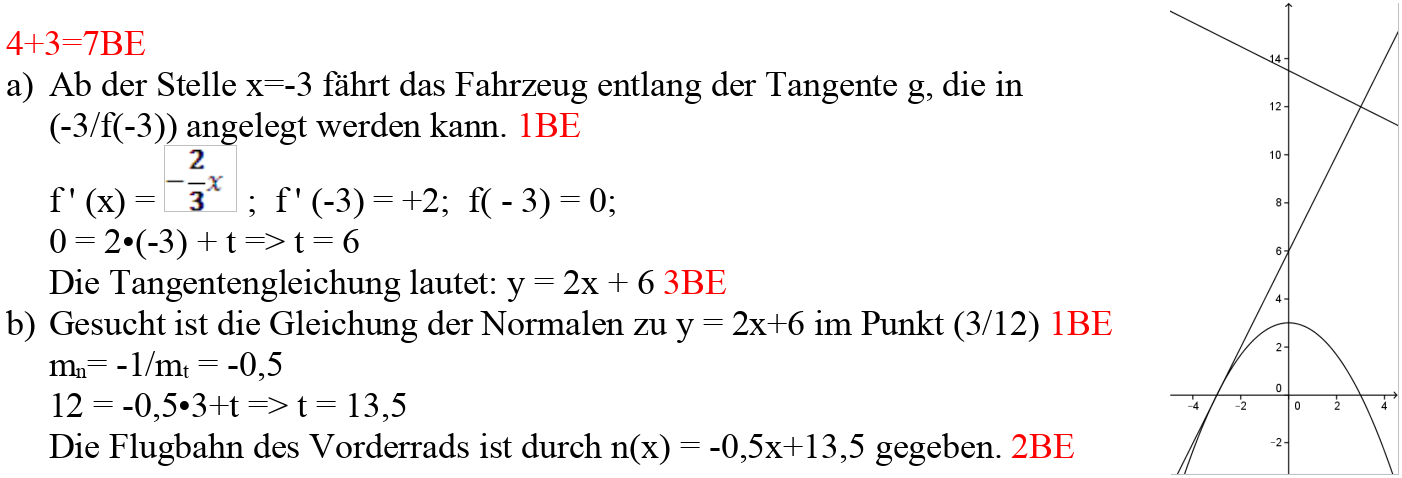
\includegraphics[width=\linewidth]{Q11_1KlausurJanuar2022_ml5.png}


%%%%%%%%%%%%%%%%%%%%%%%%%%%%%%%%%%%%%%%%%%%%%%%%%%%%%%
%%%%%%%%%%%%%%%%%%%%%%%%%%%%%%%%%%%%%%%%%%%%%%%%%%%%%%
\end{document}
